\documentclass[a4paper,12pt]{article}

\RequirePackage{epsfig}
\usepackage{todonotes}
\usepackage{pgfgantt}
\usepackage{adjustbox}
\usepackage{parskip}
\usepackage[colorlinks=true, linkcolor=blue, citecolor=blue, urlcolor=blue]{hyperref}
\usepackage{pgfgantt}
\usepackage{geometry}
\usepackage{xcolor}

\setlength{\parindent}{0pt}
\setlength\hoffset{-0.5in}      %% these work quite well with a 12pt font
\setlength\voffset{-0.5in}
\setlength{\textwidth}{6.30in}
\setlength{\textheight}{9.0in}
\bibliographystyle{unsrt}

\begin{document}

\begin{center}
{\Large\bf{Evaluating Contrastive Explanations}} \\
      \vspace{5.0mm}
{\Large\bf{Project Plan}} \\
      \vspace{8mm}
      {\large\bf{52093275}}  \\
      \vspace{5.0mm}
      \vspace{8mm}
      {\large\bf{Hariss Ali Gills}}  \\
      \vspace{5.0mm}
       {\tt h.gills.20@abdn.ac.uk} \\
      \vspace{5.0mm}
      {\em Department of Computing Science,\\
       University of Aberdeen, Aberdeen AB24 3UE, UK} 
\end{center}


\section*{Introduction}
Machine learning (ML) models are increasingly utilized to support major decisions in various industries \cite{angra2017machine}. These models may be Black Box Models which cannot be understood by looking at their parameters (e.g. a neural network). However, the field of Explainable Artificial Intelligence (XAI) attempts to address this issue by understanding models and their predictions to promote efficient debugging of models and to achieve a higher degree of user satisfaction and trust \cite{molnar2020interpretable}. One such method is through Counterfactuals (CF) explanations which suggest what should be different in the input instance to flip the outcome. This in turn, leads to a Contrastive explanation, focusing on the differences in features that led to the different outcome.

CF explanations are fundamental in closing the gap between the users' mental model and the ML prediction \cite{miller2019explanation}. For example, a customer of a bank using a ML-powered loan approval system that has been rejected can take the necessary steps to take action. Likewise, a bank would want to know its model is in line with financial regulation. Miller et al's work also concluded that good explanations, in addition to being contrastive, are selected in a biased manner and that they are socially aligned \cite{miller2019explanation}. A survey on the latest CF methods by Guidotti et al. presented a taxonomy of CF explainers and quantitatively benchmarked these explainers on several metrics \cite{guidotti2024counterfactual}.

This dissertation aims to use a number of the metrics defined in the survey to statistically compare the following methods:

\begin{itemize}
\item Diverse Counterfactual Explanations (DICE) is an optimization-based CF method that ensures feasibility and diversity while finding counterfactuals \cite{mothilal2020explaining}. It was found to be a top performer on most of the metrics in the survey \cite{guidotti2024counterfactual}.  
\item Artificial Immune Diverse Explanations (AIDE) is another optimization-based CF method which uses the Immune System as a metaphor to find the counterfactuals \cite{forrest2021contrastive}. This method was adapted from the opt-aiNet algorithm \cite{brownlee2011clever} inspired by the clonal selection theory of acquired immunity. 
\end{itemize}

\section*{Goals}
As mentioned in the introduction, the goal of the paper is to conduct an experiment to statistically compare DICE and AIDE. Specifically, based on the following metrics chosen based on their importance:

\begin{itemize}
\item Size: Measures the proportion of counterfactuals generated relative to the maximum requested, emphasizing the ability to produce multiple explanations when applicable. Higher values are better.
\item Dissimilarity: Evaluates the proximity between the original instance and the counterfactuals, considering both feature-level sparsity and overall distance. Lower values are better.
\item Runtime: measures the efficiency based on the elapsed time needed for the explainer to generate counterfactuals. A shorter runtime indicates better performance.
\item Actionability: Measures the proportion of counterfactuals that can be practically implemented based on actionable features; higher values indicate better actionability.
\item Diversity: Evaluates the variety among counterfactuals in terms of both feature differences and overall distance, with greater diversity being preferable.
\end{itemize}

\subsection*{Additional Goals}
The experiment can be expanded to consider the following:

\begin{enumerate}
\item Measure metrics like Instability, Implausibility, and Discriminative Power.
\item Develop a version of AIDE that is optimized for a certain metric.
\item Compare counterfactuals from different domains to check if counterfactuals perform better in some domains than others.
\item Compare counterfactuals from different Black Box Models to see if counterfactuals perform better in specific models.
\end{enumerate}



\section*{Methodology}
In addition to iteratively working on the project report, the following steps will be taken to achieve the goals:

\begin{itemize}
\item Reading the background work and understanding DICE, AIDE, and the experimental design of the survey.
\item Preprocess the \verb|adult|, \verb|compas|, \verb|fico|, and \verb|german| datasets since they are common in XAI literature.
\item Train and tune the hyperparameters of Random Forest and Deep Neural Network classifiers for each dataset. 
\item Statistically evaluate and plot the results of the measured metrics.
\end{itemize}

\section*{Resources Required}
To develop the project, the following resources are required:

\begin{itemize}
\item A machine with a web browser, an internet connection, and a text editor.
\item \verb|Python 3.11+|
\item The \verb|dice_ml| package and its dependencies like \verb|sklearn|, \verb|keras|, \verb|tensorflow|. 
\end{itemize}

\section*{Risk Assessment}
Time constraints represent a significant risk factor that may impede the completion of the project. To address this challenge, the number of metrics, model types, and datasets will be reduced. Such adjustments will allow for a more focused and manageable approach. Since a majority of the datasets cover socially sensitive tasks, consulting with experts from relevant domains valuable insights and ensure that the counterfactuals align with professional and ethical standards.

%\newpage
\section*{Timeline}
\begin{figure}[h]
    \centering
    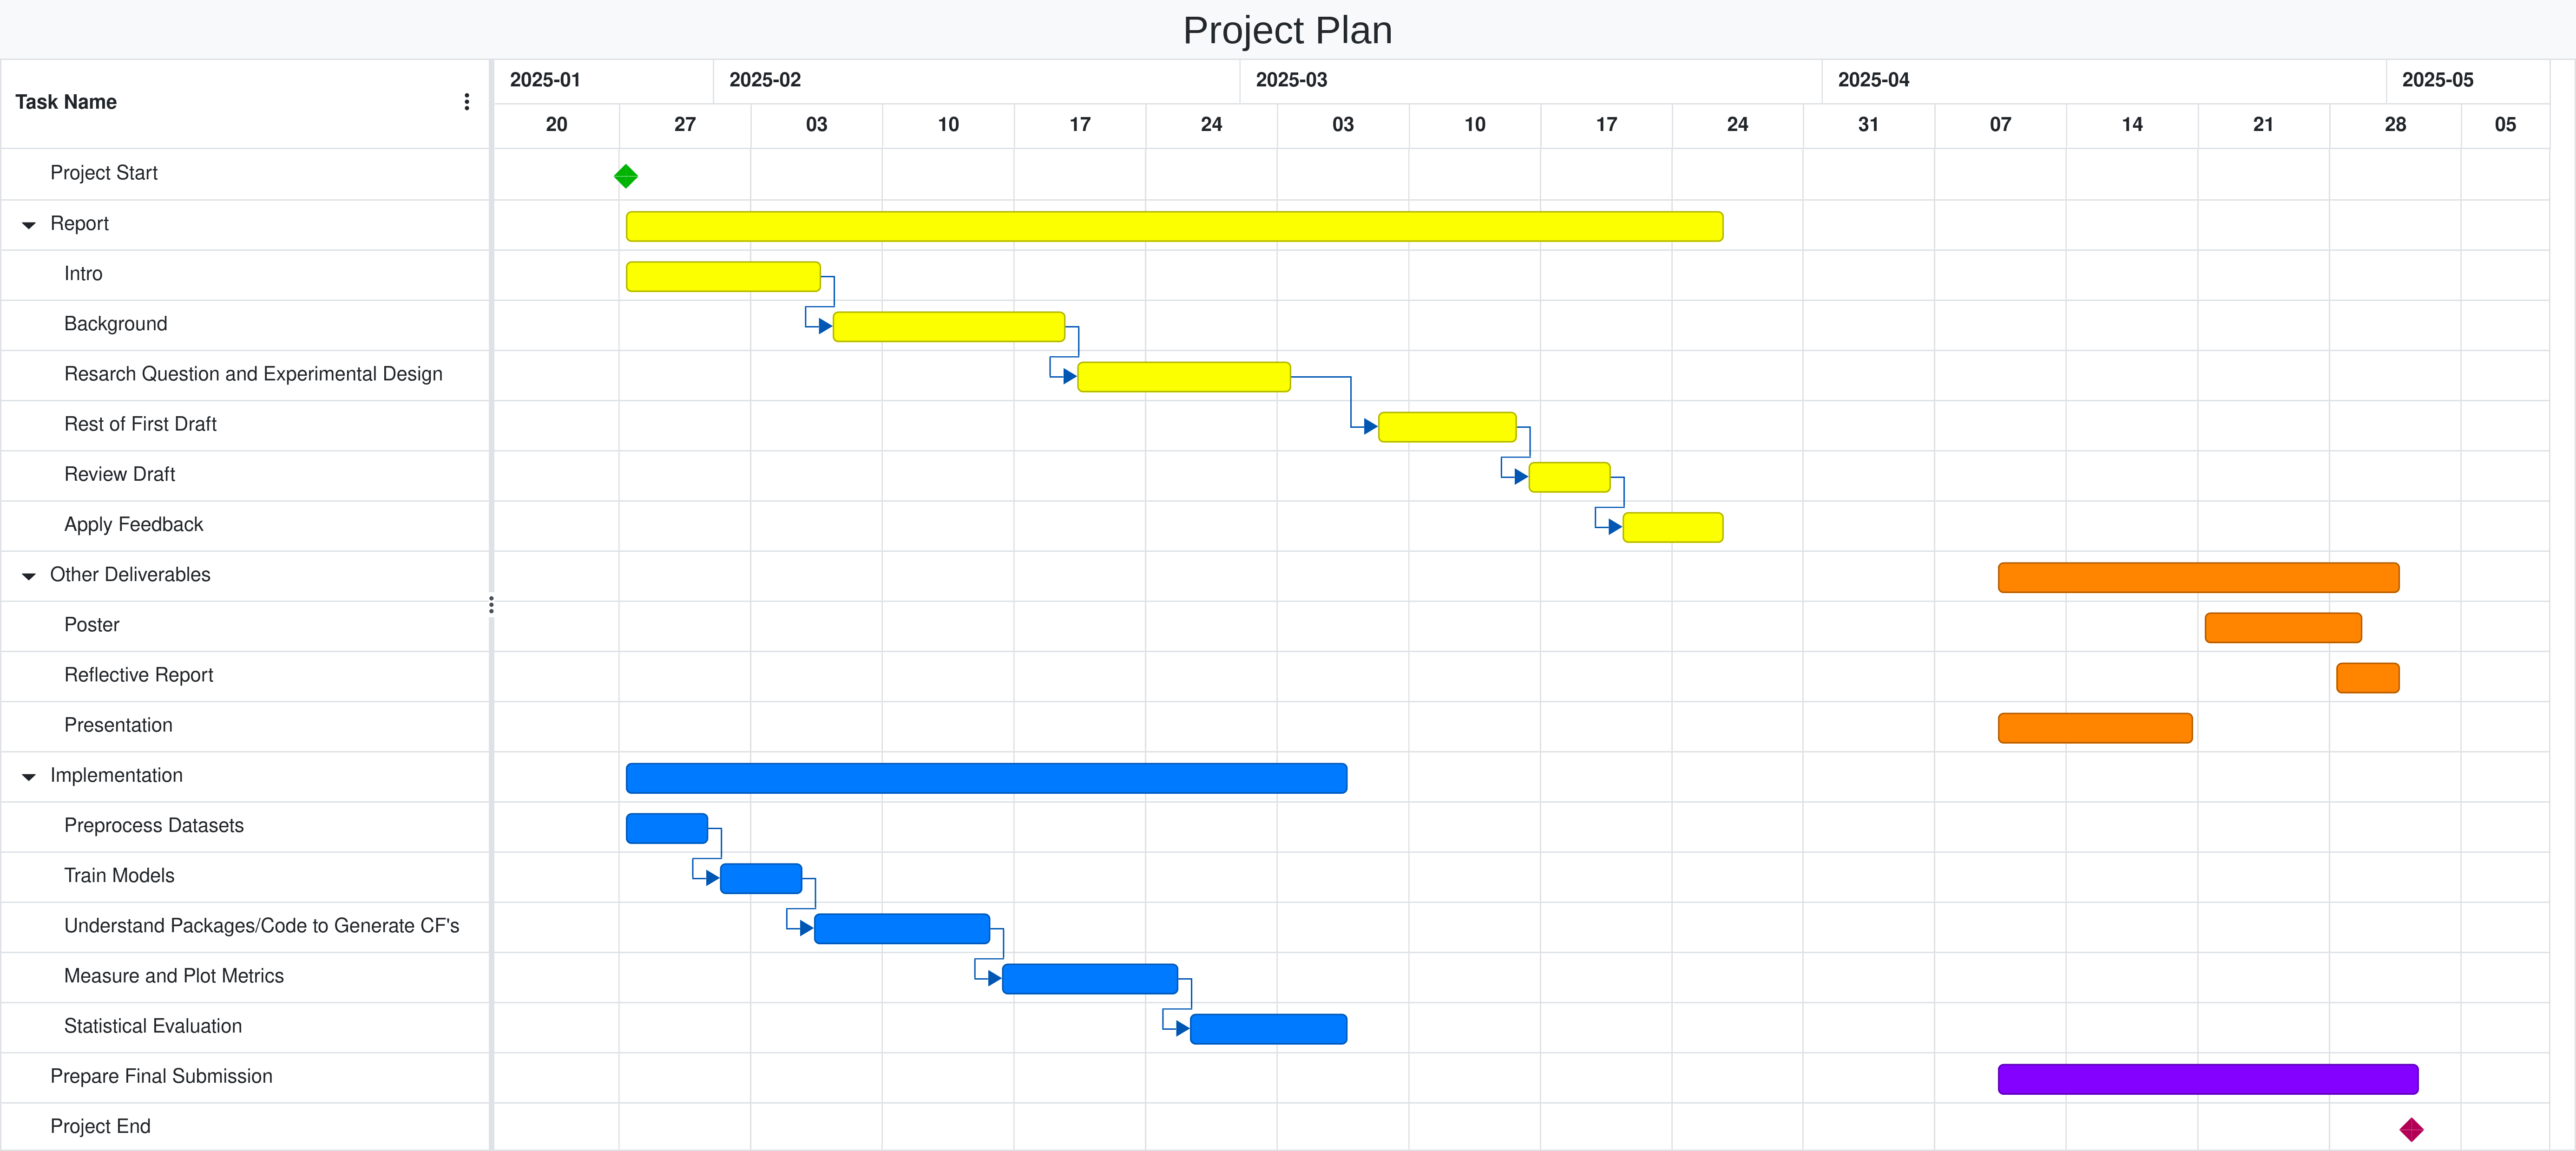
\includegraphics[width=1\textwidth]{gnatt-chart.png}
    \caption{Project Gantt Chart}
    \label{fig:gantt_chart}
\end{figure}
\bibliography{abdn-plan}

\end{document}
